\documentclass[article]{IEEEtran}

\usepackage{cite}
\usepackage{amsmath,amssymb,amsfonts}
\usepackage{algorithmic}
\usepackage{graphicx}
\usepackage{textcomp}
\usepackage{xcolor}
\usepackage{flushend}
\usepackage{listings}

\usepackage[utf8]{inputenc}
\def\BibTeX{{\rm B\kern-.05em{\sc i\kern-.025em b}\kern-.08em
    T\kern-.1667em\lower.7ex\hbox{E}\kern-.125emX}}
\begin{document}

\title{Processamento de Streams\\Análise a Corridas de Táxis}


\author{\IEEEauthorblockN{André Lopes}
\IEEEauthorblockA{\textit{Departamento de Informática} \\
\textit{Faculdade de Ciências e Tecnologia da Universidade Nova de Lisboa }\\
Almada, Portugal}

\and
\IEEEauthorblockN{Nelson Coquenim}
\IEEEauthorblockA{\textit{Departamento de Informática} \\
\textit{Faculdade de Ciências e Tecnologia da Universidade Nova de Lisboa }\\
Almada, Portugal}
}

\maketitle



\section{Introdução}

\section{\textit{Frequent Routes}}

O objectivo deste \textit{query} é achar o top 10 das rotas mais frequentes durante um período de 30 minutos. Um rota é representada por uma \textit{cell} inicial e uma \textit{cell} final.

Na Figura \ref{fig:frequentRoutesDiagram} observa-se a estrutura desta query. Primeiramente efetua-se uma janela deslizante de 30 minutos sobre o input. De seguida, seleciona-se os 10 resultados com a frequência mais alta.

\begin{figure}[hbtp]
    \centering
        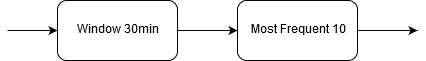
\includegraphics[width=0.5\textwidth]{images/frequentRoutesDiagram}
    \caption{Diagrama da query \textit{Frequent Routes}.}
    \label{fig:frequentRoutesDiagram}
\end{figure}

O código siddhi que implementa esta \textit{query} é o seguinte:

\begin{lstlisting}[language=SQL]
from TaxiSecStr#window.time(30 minutes)
select pickup_grid_x, pickup_grid_y, 
	dropoff_grid_x, dropoff_grid_y,
	count(*) as frequency
group by pickup_grid_x, pickup_grid_y,
 dropoff_grid_x, dropoff_grid_y
order by frequency DESC
insert into RouteFrequencyStr;

from RouteFrequencyStr#window.length(10)
select *
insert into TopFreqRoutesStr;
\end{lstlisting}


\section{\textit{Profitables Areas}}

Nesta query pretende-se identificar, de forma contínua, as áreas que são mais lucrativas para os taxistas. Para tal, o lucro de uma área é definido pelas receitas geradas nessa área a dividir pelo número de táxis vazios também nessa área.

A receita gerada numa área é a média das \textit{fare} + \textit{tip} de todas as corridas que originaram nessa área e que acabaram nos 15 minutos seguintes.

O número de táxis vazios é a soma dos táxis que efetuaram uma \textit{dropoff} nessa área mas que após 30 minutos ainda não efetuaram uma \textit{pickup}.

Na Figura \ref{fig:profitablesAreasDiagram} pode-se observar um diagrama que demonstra o fluxo desta \textit{query}.

\begin{figure}[hbtp]
    \centering
        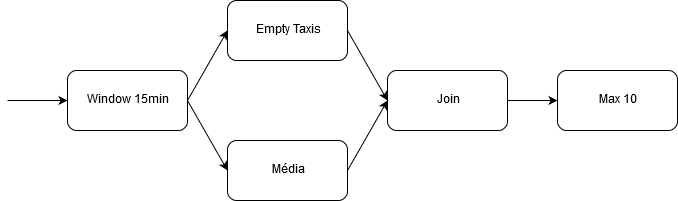
\includegraphics[width=0.5\textwidth]{images/profitableAreasDiagram}
    \caption{Diagrama da query \textit{Profitables Areas}.}
    \label{fig:profitablesAreasDiagram}
\end{figure}

O código siddhi que implementa esta \textit{query} é o seguinte:

\begin{lstlisting}[language=SQL]
from TaxiSecStr#window.time(15 min)
select avg(FareTrip)
group by pickup_grid_x, pickup_grid_y,
   dropoff_grid_x, dropoff_grid_y
insert into ProfitStr;

verificar esta query no paper esta diferente
from e1 = TaxiSecStr ->
   TaxiSecStr[e1.medallion == medallion 
   and pickup_datetime - e1.dropoff_datetime > 30 mins]
select * 
insert into EmptyTaxisStr 
\end{lstlisting}

\section{Idle Taxis}
\begin{lstlisting}[language=SQL]
from TaxiSecStr#window.time(1 hour)
select *
insert into AvailableTaxisStr;

from e1 = TaxiSecStr -> 
   e2 = TaxiSecStr[e2.medallion == e1.medallion]
select e1.medallion as taxi, 
(e2.pickup_datetime 
   - e1.dropoff_datetime) as idle_time
insert into IdleTimeTaxisStr;


// idle_time is in seconds
from IdleTimeTaxisStr#window.time(1 hour)
select taxi, avg(idle_time)
insert into IdleTaxisStr;
\end{lstlisting}
\section{Congested Areas}
\begin{lstlisting}[language=SQL]
from every e1 = TaxiSecStr,
   e2 = TaxiSecStr[e2.medallion 
   		== e1.medallion 
	and e2.ride_duration 
		> e1.ride_duration],
   e3 = TaxiSecStr[e3.medallion 
   		== e2.medallion 
	and e3.ride_duration 
		> e2.ride_duration],
   e4 = TaxiSecStr[e4.medallion 
   		== e3.medallion
    and e4.ride_duration 
    	> e3.ride_duration]
select e1.medallion as medallion,
 	e1.pickup_grid_x as grid_x, 
 	e1.pickup_grid_y as grid_y
insert into CongestedAreasStr;
\end{lstlisting}

\section{Most Pleasant Taxi Drivers}

\begin{lstlisting}[language=SQL]
from TaxiSecStr
select dropoff_day, hack_license as driver,
	sum(tip_amount) as tips_total
group by dropoff_day, hack_license
order by tips_total DESC
insert into DriversTipsPerDay;
\end{lstlisting}

\section{Conclusão} 


\bibliography{bibliography}

\bibliographystyle{IEEEtran}
\end{document}
